\documentclass[times,11pt]{article} %%Margins must be 1 inch, top & bottom 1 in%%
\usepackage[small,compact]{titlesec}
\usepackage{verbatim}
\usepackage{wrapfig}

\marginparwidth 0pt
\oddsidemargin  0pt
\evensidemargin  0pt
\marginparsep 0pt
\topmargin   -.50in
\textwidth   6.5in
\textheight  9in



\usepackage[pdftex]{graphicx}
\bibliographystyle{unsrt}
\usepackage{url}

\usepackage[usenames]{color}
\definecolor{plum}  {rgb}{.6,0,.6}
\definecolor{forest}  {rgb}{0,.6,0}
\definecolor{midnight}  {rgb}{0,0,.8}
\usepackage[pdftex,plainpages=false,pdfpagelabels,colorlinks=true,urlcolor=midnight,linkcolor=midnight,citecolor=forest]{hyperref}

%\RequirePackage[colorlinks,linkcolor=forest,citecolor=blue,urlcolor=blue]{hyperref}


\newtheorem{theorem}{Theorem}
\newtheorem{lemma}{Lemma}
\newtheorem{corollary}{Corollary}
\newtheorem{definition}{Definition}
\newtheorem{conjecture}{Conjecture}

%\newcommand{\yao}[1]{{\color{blue}{#1}}}
%\newcommand{\becca}[1]{{\color{black}{#1}}}
%\newcommand{\laura}[1]{{\color{cyan}{#1}}}
%\newcommand{\todo}[1]{{\color{red}{#1}}}
\newcommand{\cf}{{\em cf.}}
\newcommand{\cX}{\mathcal{X}}
\def\htheta{{\widehat{M}}}
\def\btheta{\boldsymbol{M}}
\def\bhtheta{\widehat{\btheta}}
%\def\bx{\bm{x}}
\def\cF{{\cal F}}
\def\cR{{\cal R}}
\def\cL{{\cal L}}
\def\grad{\nabla}
\newcommand{\wh}[1]{\widehat{#1}}
\newcommand{\wt}[1]{\widetilde{#1}}
\newcommand{\Ave}[1]{\left\langle #1 \right\rangle}
\newcommand{\ave}[1]{\langle #1 \rangle}

\def\ie{{\em i.e.,~}}
\def\eg{{\em e.g.,~}}
\def\cf{{\em cf.,~}}
\def\ea{{\em et al.~}}


% *** SUBFIGURE PACKAGES ***
%\usepackage[tight,footnotesize]{subfigure}
% subfigure.sty was written by Steven Douglas Cochran. This package makes it
% easy to put subfigures in your figures. e.g., "Figure 1a and 1b". For IEEE
% work, it is a good idea to load it with the tight package option to reduce
% the amount of white space around the subfigures. subfigure.sty is already
% installed on most LaTeX systems. The latest version and documentation can
% be obtained at:
% http://www.ctan.org/tex-archive/obsolete/macros/latex/contrib/subfigure/
% subfigure.sty has been superceeded by subfig.sty.



%\usepackage[caption=false]{caption}
%\usepackage[font=footnotesize]{subfig}
% subfig.sty, also written by Steven Douglas Cochran, is the modern
% replacement for subfigure.sty. However, subfig.sty requires and
% automatically loads Axel Sommerfeldt's caption.sty which will override
% IEEEtran.cls handling of captions and this will result in nonIEEE style
% figure/table captions. To prevent this problem, be sure and preload
% caption.sty with its "caption=false" package option. This is will preserve
% IEEEtran.cls handing of captions. Version 1.3 (2005/06/28) and later 
% (recommended due to many improvements over 1.2) of subfig.sty supports
% the caption=false option directly:
\usepackage[caption=false,font=footnotesize]{subfig}
%
% The latest version and documentation can be obtained at:
% http://www.ctan.org/tex-archive/macros/latex/contrib/subfig/
% The latest version and documentation of caption.sty can be obtained at:
% http://www.ctan.org/tex-archive/macros/latex/contrib/caption/




% *** CITATION PACKAGES ***
%
\usepackage{cite}

% correct bad hyphenation here
\hyphenation{op-tical net-works semi-conduc-tor}


\newcommand{\fixme}{\textcolor{red}}
\newcommand{\laura}{\textcolor{magenta}}


\begin{document}
%
% paper title
% can use linebreaks \\ within to get better formatting as desired
\title{\vspace{-50pt}Connectome Coding}

\author{Laura Balzano \& Joshua T.~Vogelstein}
\date{}
\def \E{\mathbb E}
\def \Expect{\mathbb E}
\def \1{\mathbf 1}
\def \P{\mathrm{Pr}}
\def \R{\mathbb{R}}
\def \S{\mathcal{S}}
\def \cA{\mathcal{A}}
\def \N{p}
\def \reals{\mathbb{R}}
\newcommand{\deq}{\mathrel{\stackrel{\scriptscriptstyle\Delta}{=}}}


\newenvironment{squishlist}
{   \begin{list}{$\bullet$}
    { \setlength{\itemsep}{2pt}      \setlength{\parsep}{2pt}
      \setlength{\topsep}{0pt}       \setlength{\partopsep}{0pt}
      \setlength{\leftmargin}{1.5em} \setlength{\labelwidth}{1em}
      \setlength{\labelsep}{0.5em} } }
      {\end{list}}
      
\newenvironment{squishlist2}
{   \begin{list}{$\blacktriangleright$}
    { \setlength{\itemsep}{2pt}      \setlength{\parsep}{2pt}
      \setlength{\topsep}{0pt}       \setlength{\partopsep}{0pt}
      \setlength{\leftmargin}{1.5em} \setlength{\labelwidth}{1em}
      \setlength{\labelsep}{0.5em} } }
      {\end{list}}



\renewcommand\thepage{C-1}


\maketitle

\subsubsection*{Challenge, Impact and Innovation}

A human brain is perhaps the most complex grapefruit sized object in the known universe, with $\mathcal{O}(10^8)$ neurons and $\mathcal{O}(10^{13})$ synapses \cite{??}.   Moreover,  magnetic resonance imaging (MRI) provides access to the living brain at high spatiotemporal resolution, $\sim$$1$ mm$^3$ and $\sim$$1$ Hz.  Yet, after 30 years of well-funded research, there remains to be a single clinically useful brain imaging based biomarker for any psychiatric diagnosis \cite{APA}. 
% 
Evidence is building that most psychiatric disorders are fundamentally ``connectopathies'', that is, disorders of connectivity \cite{??}. Based on this, 
\textbf{we conjecture that the lack of clinically useful brain imaging biomarkers stems from an absence of adequate statistical models of brain connectivity.} More specifically, both functional and diffusion MRI data can yield estimates of human brain connectivity, or ``connectomes''.  The challenge is to build statistical models linking brain connectivity to phenotype.  Learning such mappings requires overcoming both computational and statistical bottlenecks.

% 
\textbf{We propose to develop statistical network models specifically for populations of networks. }  This is in stark contrast to nearly all extant models of networks, which typically model a single network (for example, the Facebook network), rather than populations thereof.  While models of populations of other data types are prevalent in neuroscience (such as population activity), we are unaware of any such population models of networks.



\subsubsection*{Rationale}

Neural coding is a rich field devoted to understanding the relationship between neural \emph{activity} and perception.  By analogy, connectome coding will become a bourgeoning field devoted to understanding the relationship between neural \emph{connectivity} and experience.  Indeed, since the days of Hebb \cite{??}, neuroscientists have conjectured that memories and experiences are stored in the connectivity patterns of the brain.  If the brain stores memories in the physical connections, then it can be free to exhibit whatever pattern it so desires, without fearing a radical reconfiguration of its memories.  On the other hand, if experience is somehow stored in ongoing activity, a sudden change of state (for example, by a seizure), could erase all history, like a etch-a-sketch.   Thus, we are motivated to build and understand models of brain connectivity. 



\begin{wrapfigure}{r}{0.42\textwidth}
%\begin{figure}[htb]
\centering
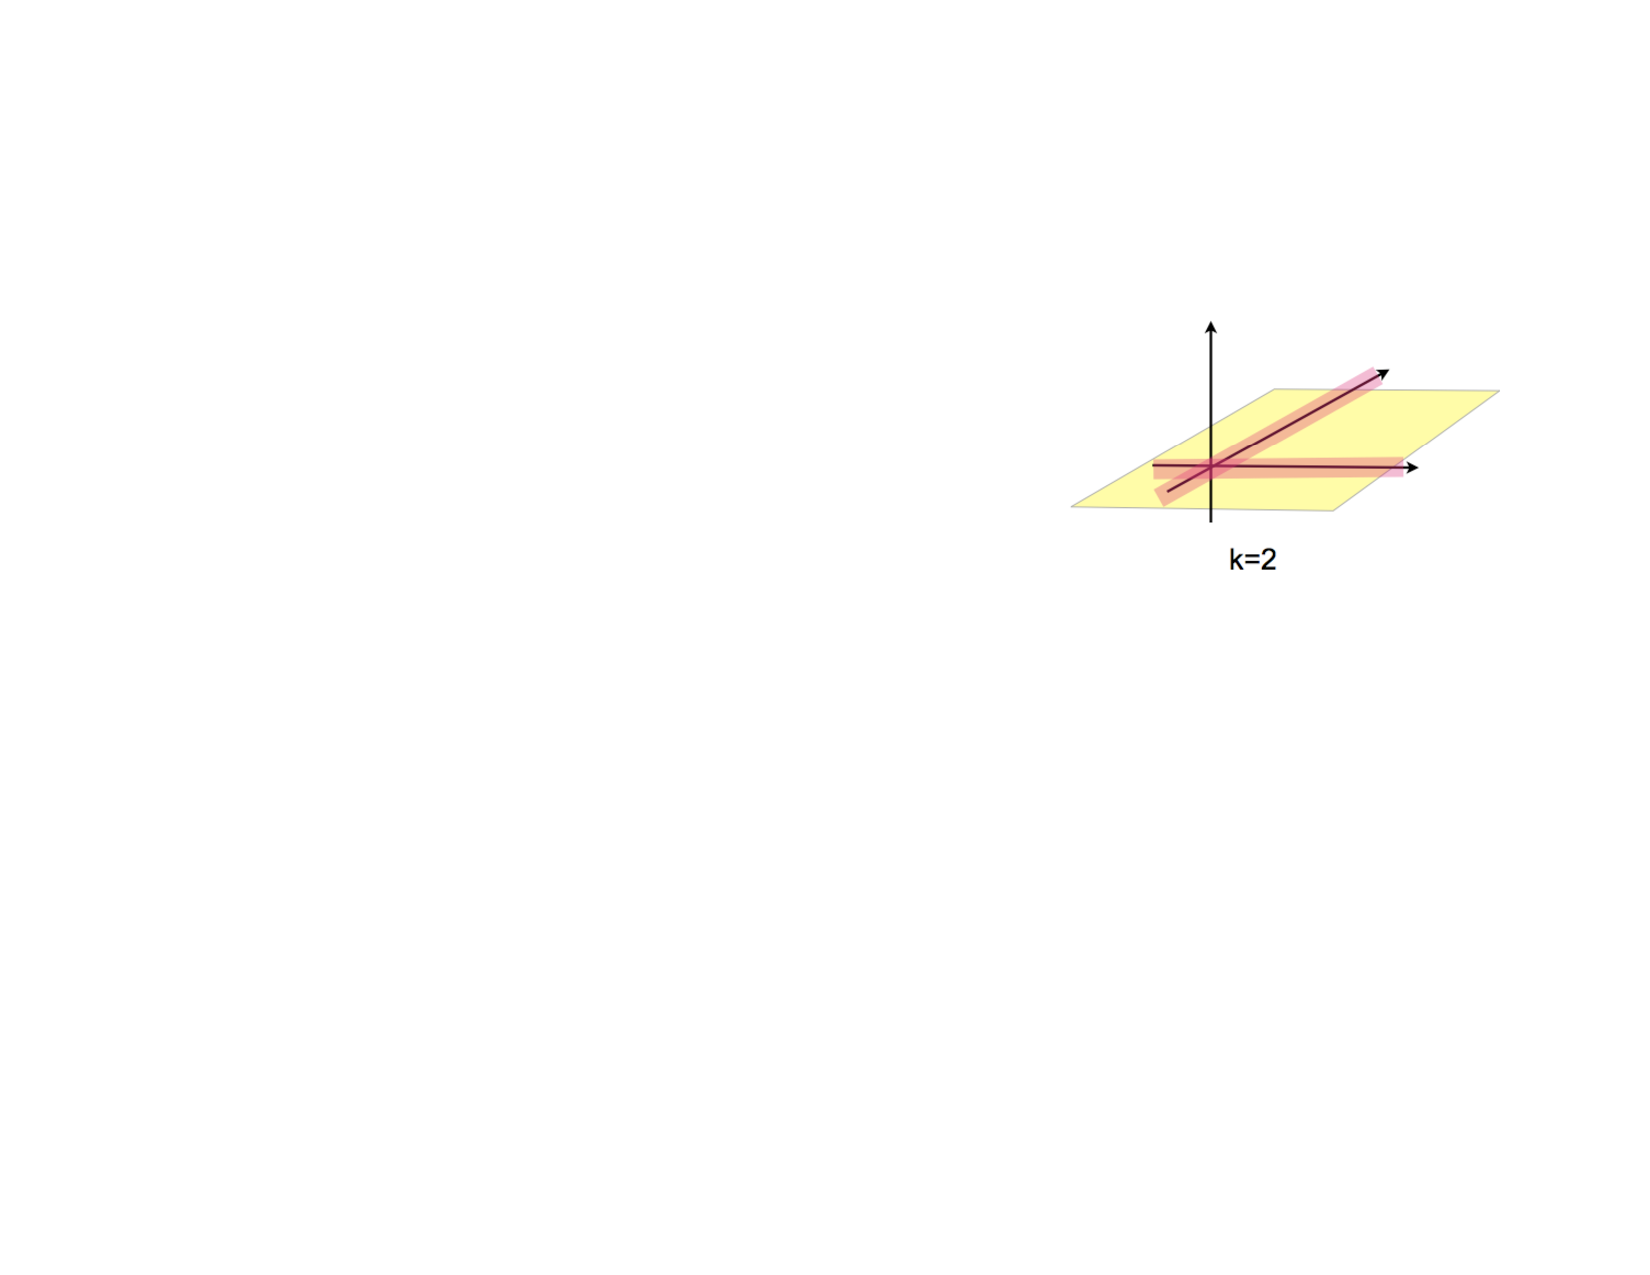
\includegraphics[width=.4\textwidth]{figs/unionspic}
\caption{\small Illustration of two 1-d subspaces and one 2-d subspace; though the two pink lines (two one-dimensional subspaces) are a simpler model than the yellow two-dimensional plane, the set they define is non-convex.}
\label{fig:unionsum}
%\end{figure}
\end{wrapfigure}



\clearpage
\paragraph{Aims}

\begin{enumerate}
	\item Models of individual connectomes
	\item Models of populations of connectomes
	\item Models relating populations of connectomes to phenotypes
\end{enumerate}



 

\newpage


\paragraph{Subspace Clustering}

Modeling data as a union of subspaces is a simple and flexible model that fits well to the context of brain-graphs.  Algorithmically, the problem of estimating the union of subspaces from data defines the problem of \emph{Subspace Clustering}, or clustering vectors into groups that lie in or near the same subspace. 


Let $A_G$ be a $n \times n$ adjacency matrix of graph $G$, where $A_{uv}=1$ iff $(u \sim v) \in \mathcal{E}_G$. 
The goal of subspace clustering is to jointly infer the underlying subspaces from $A$ and to cluster the vertices of $A$ according to their corresponding subspaces. This would in turn give us an understanding of potential clusters of connectivity. From our preliminary results, subspace clustering is a much better tool for clustering connectivity than spectral clustering of the graph or activity, or anatomical clustering, which is the state-of-the-art approach \cite{}. There are three open problems that we wish to address.

\section{Spectral Clustering versus Subspace Clustering}

This is our first theoretical contribution. The connections are clear in certain problems, give example.

\section{Subspace Clustering Analysis} Understanding the theoretical properties of the subspace clustering algorithm is crucial to creating better statistical tests for brain connectivity. The current state-of-the-art algorithms rely heavily on \laura{more here and...}


\paragraph{Algorithmic Analysis} The subspace clustering problem is non-convex and finding an optimal solution to the subspace clustering problem is NP-hard \cite{vidaltutorial}. However, it is believed that under mild conditions separating the subspaces, properly initialized simple algorithms like the EM algorithm should provably succeed in identifying the true subspaces underlying the data. A second theoretical contribution of our work will be to pursue this theorem of algorithmic global convergence.

\laura{Laura will talk here about avenues we could pursue. }

\paragraph{Statistical Analysis} Consistency, of course.



\section{Missing-Data Subspace Clustering (or general aspects of the reality of data)}


Low-rank matrix completion allows one to estimate a single subspace from incomplete data, and this work has recently been extended for the subspace clustering problem~\cite{hrmc, balzano2012ssp, pimentel2014}. However, the algorithm analyzed in~\cite{hrmc} is computationally demanding and intractable in the number of clusters. While the algorithms in~\cite{balzano2012ssp, pimentel2014} are computationally efficient, they have no convergence guarantees. 




\begin{enumerate}
\item Adapting the brain region clustering problem to the framework of subspace clustering, and studying the similarities and differences to the spectral clustering approach.
\item Analyzing the subspace clustering algorithm in this context, which we expect to result in both algorithmic and statistical convergence guarantees.
\item \laura{Something else here, like perhaps dealing realities of actual brain data, applying it, maybe missing data and corruptions, etc.}
\end{enumerate}



\setcounter{page}{1}
\renewcommand\thepage{F-\arabic{page}}
\bibstyle{alpha}
\bibliography{pecase}

% that's all folks
\end{document}


